\documentclass[journal,12pt,twocolumn]{IEEEtran}
\usepackage{setspace}
\usepackage{gensymb}
\usepackage{xcolor}
\usepackage{caption}
\singlespacing
\usepackage{siunitx}
\usepackage[cmex10]{amsmath}
\usepackage{mathtools}
\usepackage{hyperref}
\usepackage{amsthm}
\usepackage{mathrsfs}
\usepackage{txfonts}
\usepackage{stfloats}
\usepackage{cite}
\usepackage{cases}
\usepackage{subfig}
\usepackage{longtable}
\usepackage{multirow}
\usepackage{enumitem}
\usepackage{mathtools}
\usepackage{listings}
\usepackage{tikz}
\usetikzlibrary{shapes,arrows,positioning}
\usepackage{circuitikz}
\let\vec\mathbf
\DeclareMathOperator*{\Res}{Res}
\renewcommand\thesection{\arabic{section}}
\renewcommand\thesubsection{\thesection.\arabic{subsection}}
\renewcommand\thesubsubsection{\thesubsection.\arabic{subsubsection}}

\renewcommand\thesectiondis{\arabic{section}}
\renewcommand\thesubsectiondis{\thesectiondis.\arabic{subsection}}
\renewcommand\thesubsubsectiondis{\thesubsectiondis.\arabic{subsubsection}}
\hyphenation{op-tical net-works semi-conduc-tor}

\lstset{
language=Python,
frame=single, 
breaklines=true,
columns=fullflexible
}
\begin{document}
\theoremstyle{definition}
\newtheorem{theorem}{Theorem}[section]
\newtheorem{problem}{Problem}
\newtheorem{proposition}{Proposition}[section]
\newtheorem{lemma}{Lemma}[section]
\newtheorem{corollary}[theorem]{Corollary}
\newtheorem{example}{Example}[section]
\newtheorem{definition}{Definition}[section]
\newcommand{\BEQA}{\begin{eqnarray}}
        \newcommand{\EEQA}{\end{eqnarray}}
\newcommand{\define}{\stackrel{\triangle}{=}}
\newcommand{\myvec}[1]{\ensuremath{\begin{pmatrix}#1\end{pmatrix}}}
\newcommand{\mydet}[1]{\ensuremath{\begin{vmatrix}#1\end{vmatrix}}}

\bibliographystyle{IEEEtran}
\providecommand{\nCr}[2]{\,^{#1}C_{#2}} % nCr
\providecommand{\nPr}[2]{\,^{#1}P_{#2}} % nPr
\providecommand{\mbf}{\mathbf}
\providecommand{\pr}[1]{\ensuremath{\Pr\left(#1\right)}}
\providecommand{\qfunc}[1]{\ensuremath{Q\left(#1\right)}}
\providecommand{\sbrak}[1]{\ensuremath{{}\left[#1\right]}}
\providecommand{\lsbrak}[1]{\ensuremath{{}\left[#1\right.}}
\providecommand{\rsbrak}[1]{\ensuremath{{}\left.#1\right]}}
\providecommand{\brak}[1]{\ensuremath{\left(#1\right)}}
\providecommand{\lbrak}[1]{\ensuremath{\left(#1\right.}}
\providecommand{\rbrak}[1]{\ensuremath{\left.#1\right)}}
\providecommand{\cbrak}[1]{\ensuremath{\left\{#1\right\}}}
\providecommand{\lcbrak}[1]{\ensuremath{\left\{#1\right.}}
\providecommand{\rcbrak}[1]{\ensuremath{\left.#1\right\}}}
\theoremstyle{remark}
\newtheorem{rem}{Remark}
\newcommand{\sgn}{\mathop{\mathrm{sgn}}}
\newcommand{\rect}{\mathop{\mathrm{rect}}}
\newcommand{\sinc}{\mathop{\mathrm{sinc}}}
\providecommand{\abs}[1]{\left\vert#1\right\vert}
\providecommand{\res}[1]{\Res\displaylimits_{#1}}
\providecommand{\norm}[1]{\lVert#1\rVert}
\providecommand{\mtx}[1]{\mathbf{#1}}
\providecommand{\mean}[1]{E\left[ #1 \right]}
\providecommand{\fourier}{\overset{\mathcal{F}}{ \rightleftharpoons}}
\providecommand{\ztrans}{\overset{\mathcal{Z}}{ \rightleftharpoons}}
\providecommand{\system}[1]{\overset{\mathcal{#1}}{ \longleftrightarrow}}
\newcommand{\solution}{\noindent \textbf{Solution: }}
\providecommand{\dec}[2]{\ensuremath{\overset{#1}{\underset{#2}{\gtrless}}}}
\let\StandardTheFigure\thefigure
\def\putbox#1#2#3{\makebox[0in][l]{\makebox[#1][l]{}\raisebox{\baselineskip}[0in][0in]{\raisebox{#2}[0in][0in]{#3}}}}
\def\rightbox#1{\makebox[0in][r]{#1}}
\def\centbox#1{\makebox[0in]{#1}}
\def\topbox#1{\raisebox{-\baselineskip}[0in][0in]{#1}}
\def\midbox#1{\raisebox{-0.5\baselineskip}[0in][0in]{#1}}

\vspace{3cm}
\title{\LaTeX\ 9.10.6.7}
\author{Lokesh Surana}
\maketitle
\section*{Class 9, Chapter, 10, Exercse 6.7}

Q. AC and BD are chords of a circle which bisect each other. Prove that (i) AC and BD are diameters, (ii) ABCD is a rectangle.

\solution
Let point $O = \myvec{0\\0}$ be the center of circle, and 
\begin{align}
    \vec{A} &= \myvec{\cos\degree0 \\ \sin\degree0} \\
    \implies \myvec{A} &= \myvec{1 \\ 0} \\
    \vec{B} &= \myvec{\cos\degree90 \\ \sin\degree90} \\
    \implies \myvec{B} &= \myvec{0 \\ 1} \\
    \vec{C} &= \myvec{\cos\degree180 \\ \sin\degree180} \\
    \implies \myvec{C} &= \myvec{-1 \\ 0} \\
    \vec{D} &= \myvec{\cos\degree270 \\ \sin\degree270} \\
    \implies \myvec{D} &= \myvec{0 \\ -1}
\end{align}

\begin{enumerate}
    \item As it is given that chords $AC$ and $BD$ bisect each other, we have
    \begin{align}
        \vec{A} + \vec{C} &= \vec{B} + \vec{D} \\
        \myvec{1 \\ 0} + \myvec{-1 \\ 0} &= \myvec{0 \\ 1} + \myvec{0 \\ -1} \\
        \myvec{0 \\ 0} &= \myvec{0 \\ 0} 
    \end{align}
    $\implies$ both chords $AC$ and $BD$ pass through the center of the circle.
    Hence, $AC$ and $BD$ are diameters of the circle.

    \item Here the $AC$ and $BD$ i.e. the diagonals of quadrilateral bisect each other. Hence, the quadrilateral $ABCD$ is either a rectangle or a parallelogram.
    %copilot write a latex to show internal angles of a this ABCD is 90 degree, using cosines rule between sides AB and BC
    Let's check the angle between adjacent sides of this quadrilateral, i.e. $AB$ and $BC$.
    \begin{align}
        \vec{AB} = \vec{A} - \vec{B} &= \myvec{1 \\ 0} - \myvec{0 \\ 1} \\
        &= \myvec{1 \\ -1} \\
        \vec{BC} = \vec{B} - \vec{C} &= \myvec{0 \\ 1} - \myvec{-1 \\ 0} \\
        &= \myvec{1 \\ 1} \\
    \end{align}
    Let $\theta$ be the angle between $\vec{AB}$ and $\vec{BC}$, then as per cosine rule
    \begin{align}
        \cos\theta &= \frac{\vec{AB} \cdot \vec{BC}}{\norm{\vec{AB}} \norm{\vec{BC}}} \\
        &= 0 \\
        \implies \theta &= \degree90
    \end{align}
    
    Hence, the quadrilateral $ABCD$ is a rectangle.
\end{enumerate}

\begin{figure}[!htb]
    \centering
    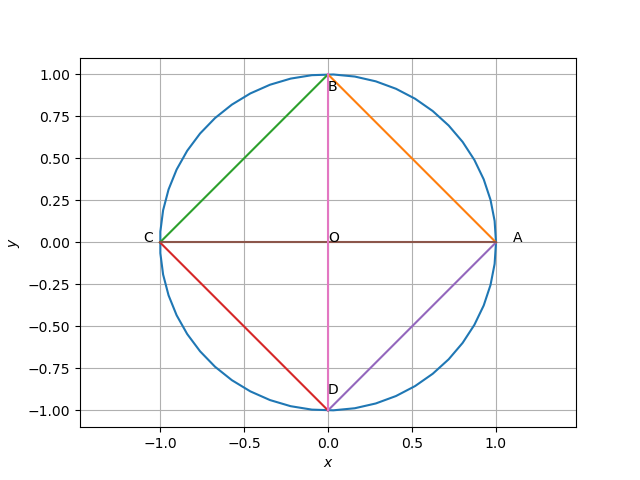
\includegraphics[width=\columnwidth]{figs/circle.png}
    \caption{circle}
    \label{fig:circle}
\end{figure}

\end{document}